\section{Методология}

Целью работы было получить размеченный корпус и обученную модель, распознающую именованные сущности. После обзора литературы были намечены задачи и работа была предварительно разделена на несколько этапов.

\begin{enumerate}
\item Получение и разметка данных
\item Обучение и тюнинг моделей
\item Сравнение результатов
\end{enumerate}

Но в течение работы по нескольким причинам были внесены корректировки. Во-первых, как я упоминала ранее в обзоре литературы, с представленными результатами в статье Невзоровой невозможно сравниваться, поскольку цели моей и их работ различаются. Во-вторых, качество полученных данных оказалось не лучшим из возможных, а алгоритм Невзоровой, разработанный как раз для разметки данных, мог бы улучшить имеющийся корпус, используемый для обучения моделей. Как следствие, было принято решение воспроизвести алгоритм из статьи Невзоровой насколько это возможно и воспользоваться полученными результатами.

\begin{enumerate}
\item Получение и разметка данных
\item Обучение и тюнинг моделей
\item Воспроизведение статьи Невзоровой
\item Разметка данных с помощью алгоритма Невзоровой
\item Обучение и тюнинг моделей
\item Сравнение результатов
\end{enumerate}


\subsection{Получение и разметка данных}

Обзор литературы показал, что существует корпус татарских текстов Туган Тел\cite{tugan_tel}. Данный копрус имеет также свою систему <<корпус-менеджер>>, которая представлена в виде сайта. На этом сайте можно искать по словоформе или лемме с огромным количеством параметров [\ref{fig:tugan_tel_1}], однако возможности просто скачать весь корпус не оказалось. Я предполагаю, что у Академии наук Республики Татарстан есть API для исполнения запросов на большом количестве данных и в каком-то более удобном формате, чем запрос на сайте, но у меня доступа к такому ресурсу нет. 

\begin{figure}
\caption{Параметры на сайте \href{http://tugantel.tatar/}{tugantel.tatar} для поиска по корпусу}
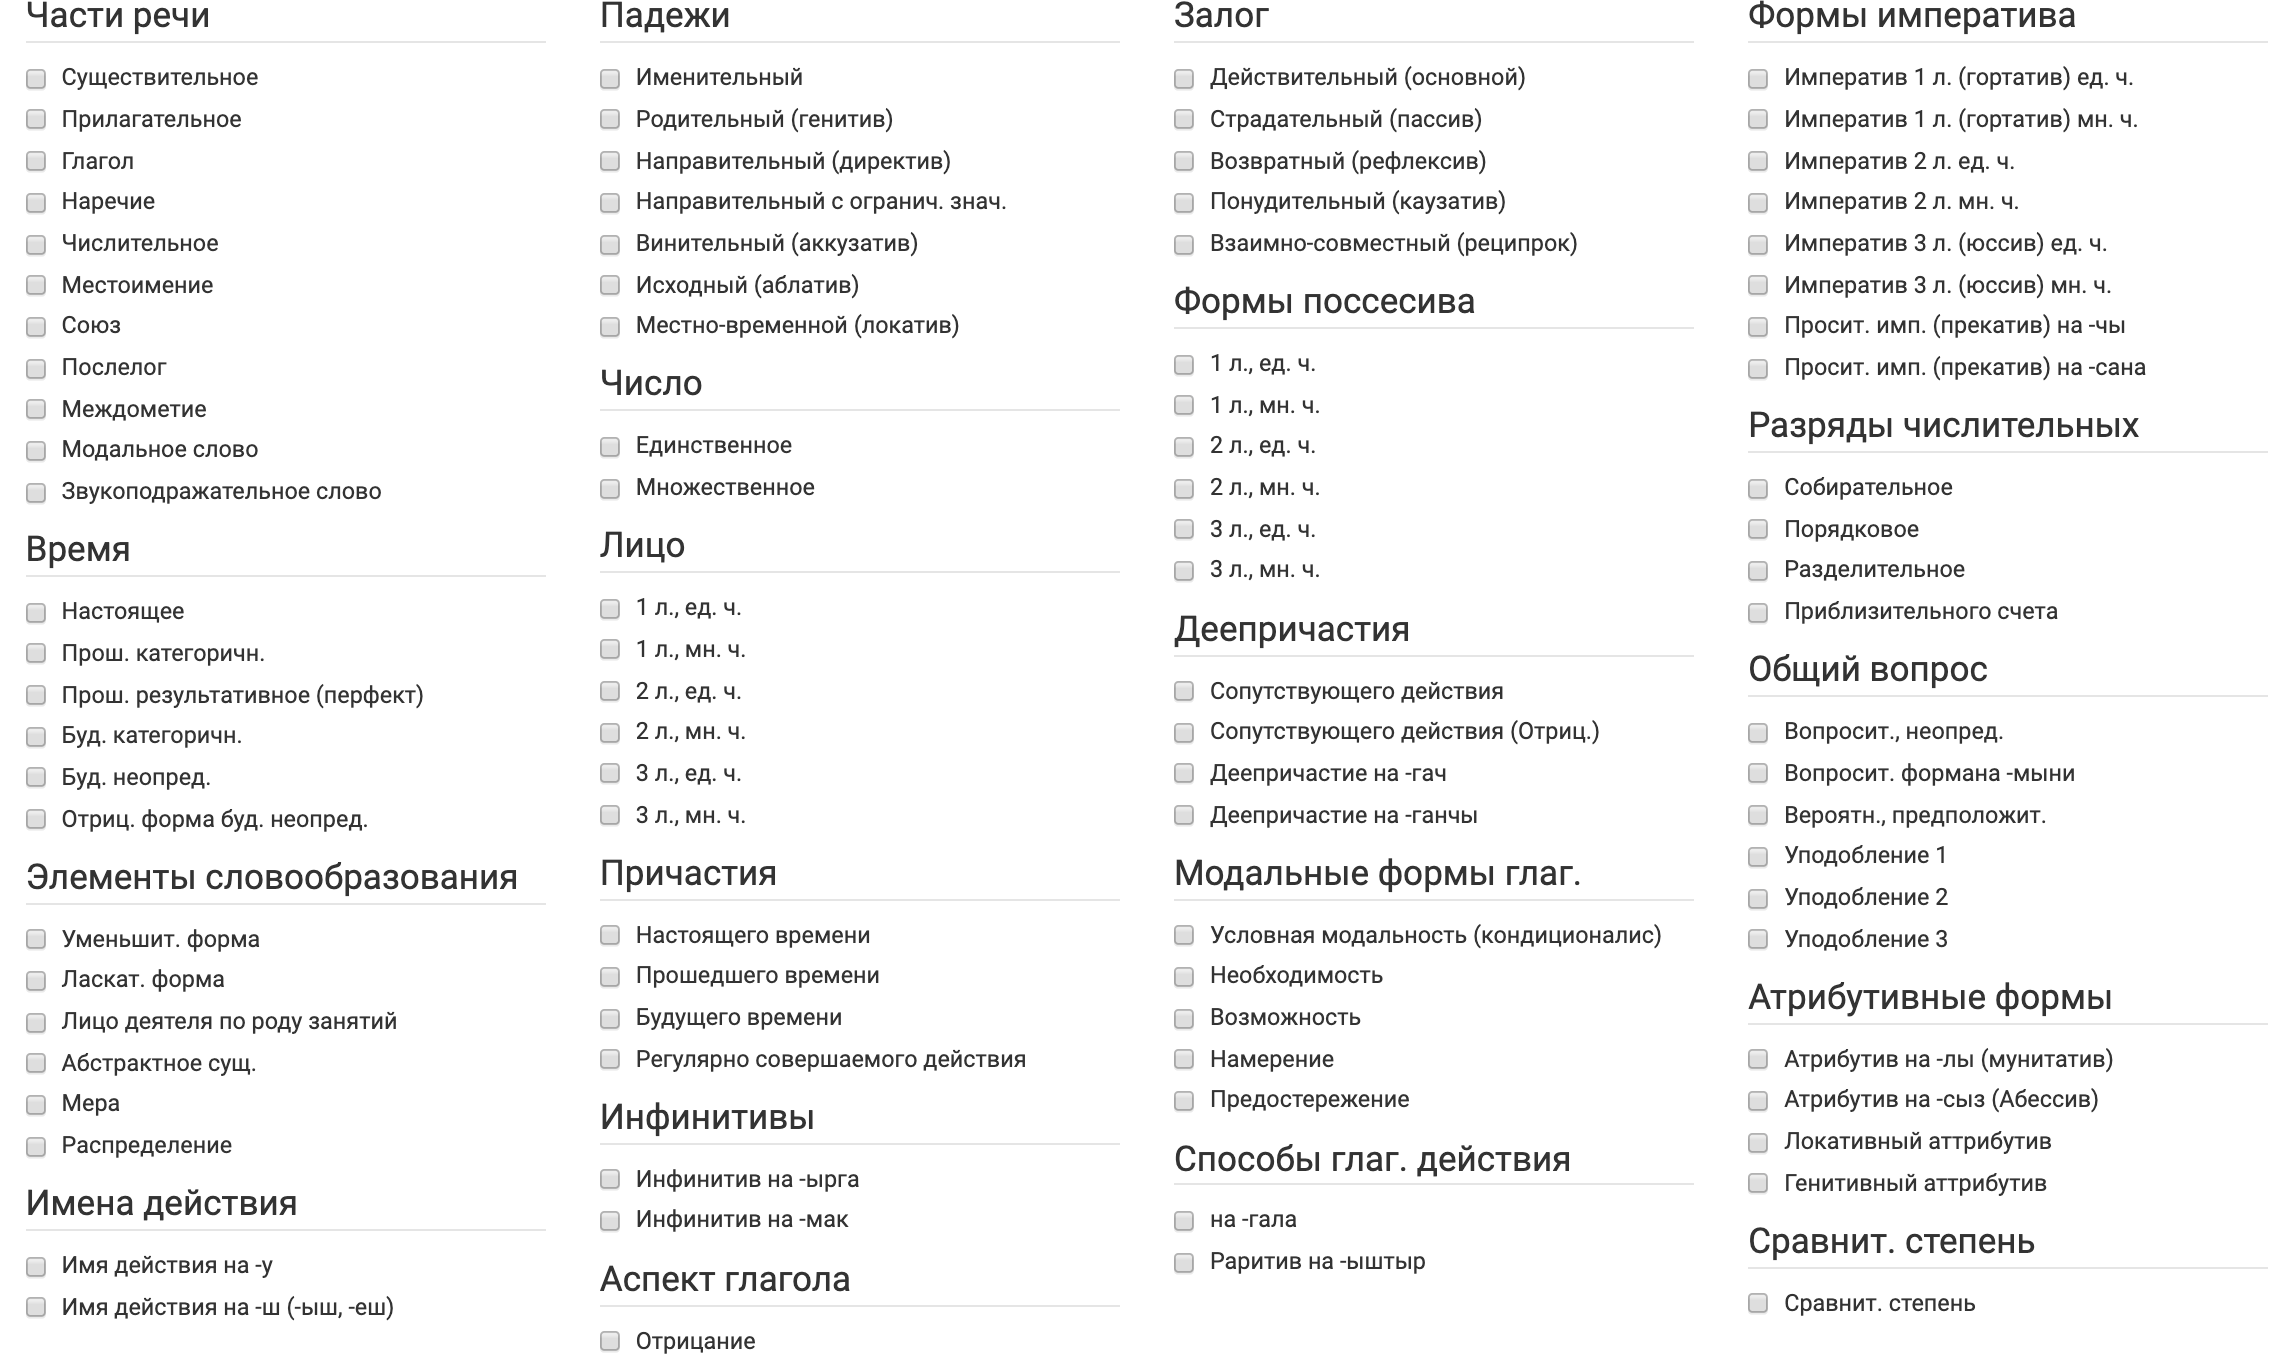
\includegraphics[width=\textwidth]{pics/tugan_tel_1}
\label{fig:tugan_tel_1}
\end{figure}


Я связалась с Невзоровой по указанной в статье электронной почте, чтобы узнать подробности об их работе и попросить о сотрудничестве. Невзорова ответила на моё письмо и предоставила мне доступ к корпусу.

Корпус представляет из себя $.zip$ файл, состоящий из $7557$ $.txt$ файлов, в общей сложности весом $1\ 183\ 023\ 978$ Б. Как уже упоминалось ранее, корпус Туган Тел автоматически размечен с помощью программного инструментарии PC-KIMMO. Разметка выглядит следующим образом: \ref{table:sample_sent} \ref{fig:sample_sent}


\begin{figure}
\caption{Пример случайного предложения из корпуса Туган Тел}
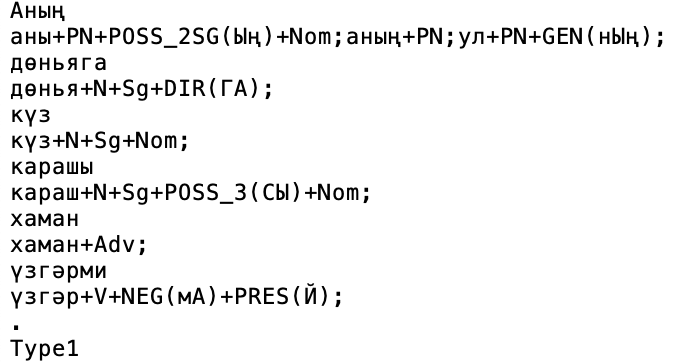
\includegraphics[width=\textwidth]{pics/sample_sent}
\label{fig:sample_sent}
\end{figure}

\begin{table}[h!]
\centering
\begin{tabular}[h]{| l | l |}
\hline
Аның & аны+PN+POSS\_2SG(Ың)+Nom;аның+PN;ул+PN+GEN(нЫң); \\
\hline
дөньяга & дөнья+N+Sg+DIR(ГА); \\
\hline
күз & күз+N+Sg+Nom; \\
\hline
карашы & караш+N+Sg+POSS\_3(СЫ)+Nom; \\
\hline
хаман &  хаман+Adv; \\
\hline
үзгәрми & үзгәр+V+NEG(мА)+PRES(Й); \\
\hline
.  & Type1 \\
\hline
\end{tabular}

Перевод: Его мировоззрение постоянно меняется.
\caption{Пример случайного предложения из корпуса Туган Тел}
\label{table:sample_sent}
\end{table}


Первое слово в каждом файле распознано как Error, все русские слова не распознаны (а их в татарском языке некоторое ненулевое количество, так как происходит какое-то достаточное количество заимствований). К сожалению для меня, очень часто русскоязычные слова оказывались как раз именованными сущностями, такими как, например, названия улиц, но распознаны они были как Error, что очень печально.

*TODO: написать \% Error от общего количества слов и привести пару примеров*

В этом файле огромная куча всяких тегов, про которые без бутылки не разберешься (и даже гугление этого парсера, блин, не помогает). Но эмпирическим методом было выяснено, что атрибут PROP --- это как раз та самая именованная сущность, что нам нужна. На основании этого все остальные атрибуты были выброшены, а PROP заменен на B-PER, так как используемая модель использовала IOB метод разметки (TODO: написать про IOB метод разметки).

Всего в текстах 30 753 824 слов, из них 534 514 это автоматически размеченные именованные сущности, что составляет $1,738\%$ от всех слов. 

*TODO: привести примеры слов с атрибутом PROP*.

*TODO: подсчитать, раз в сколько предложений в среднем встречается именованная сущность*

Также в качестве корпуса текста есть татарская википедия. На данный момент она содержит 89 252 статей, причём некоторые из них сгенерированы автоматически, что ухудшает качество текстов как корпуса для обучения, так как некоторые фразы становятся частотными не из-за того, что они действительно часто используются в языке, а из-за множества сгенерированных статей. *TODO вставить пример про бассейны*

Проблема с татарской википедией также была в смеси латиницы и кириллицы *TODO экскурс в историю по поводу того, как мы до такой жизни дошли*, так что пришлось ещё и из латиницы в кириллицу переводить.


\subsection{Обучение и тюнинг моделей}

\subsubsection{BiLSTM-CRF}

Была использована модель BiLSTM-CRF, которая норм заработала. Она использует разметку IOB, так что данные пришлось немного подкорректировать и добавить данную разметку. Весь морфологический разбор, кроме разметки именованных сущностей, никак не используется. Из-за того, что у меня нет мощностей для вычислений, приходилось обучаться не на всей выборке, а только на части. Модель показала очень хороший результат.

\medskip

\begin{tabular}{| l | l | l | l | l | l | l |}
\hline
Category               & Precision  &   Recall   &  F-score   &  Predicts  &   Golds    &  Correct   \\

\hline
 PER                                 & 99.768     & 90.727     & 95.033     & 2589       & 2847       & 2583       \\
\hline
\end{tabular}



*TODO: описание модели*

\subsubsection{BERT}

BERT есть для татарского языка, так что осталось его только запустить, что я ещё не сделала, но планирую вот уже на этой неделе. TODO: описать BERT.


\section{Воспроизведение статьи Невзоровой}

Была воспроизведена статья Невзоровой, на министерствах действительно показала хорошие результаты, но стало очевидно, что это полуручная история, потому что мусор пришлось выкидывать в ручном режиме. Ну и не удалось воспроизвести запросы в Туган Тел, а поиск был возможен только по слову (фразе). С помощью этого результата хочется разметить википедию, на википедии обучиться, а потом попытаться протестировать на Туган Тел и сравнить результаты.

\section{Сравнение результатов}

В процессе.


